\documentclass[numbers=noenddot,12pt,a4paper]{scrartcl}
\usepackage[greek,ngerman]{babel}
\usepackage[T1]{fontenc}
\usepackage[utf8]{inputenc}
\usepackage{fullpage}
\usepackage{libertine}
\usepackage{ziffer}
\usepackage{graphicx}
\usepackage{units}
\usepackage[infoshow]{tabularx}
\usepackage{amsmath}
\usepackage{amssymb}
\usepackage{wrapfig}
\usepackage{esint}
\usepackage{float}
\usepackage{wrapfig}
\usepackage[font=small]{caption}
\usepackage{subcaption}

\renewcommand{\thefigure}{Abb. \arabic{figure}}

\captionsetup[wrapfigure]{name=}
\captionsetup[figure]{name=}
\newcommand{\degree}{^\circ}
\newcommand{\diff}{\textnormal{d}}
\newcommand{\tenpo}[1]{\cdot 10^{#1}}
\newcommand{\greek}[1]{\greektext#1\latintext}
\newcommand{\ix}[1]{_\text{#1}}
\newcommand{\imag}{\mathbf{i}}
\newcommand{\tilt}[1]{\textit{#1}}
\newcommand{\grad}[1]{\textit{grad}\left(#1\right)}
\newcommand{\divergenz}[1]{\textit{div}\left(#1\right)}
\newcommand{\euler}{\mathnormal{e}}

\title{Protokoll: nanoparticle tracking}
\author{Tom Kranz, Philipp Hacker}
\date{\today}

\begin{document}
%\setcounter{page}{2}
%\setcounter{section}{1}
\maketitle
\begin{center}
Betreuer: M. Paßvogel\\
Versuchsdatum: 22.10.2014\\
\begin{table}[H]
\centering
Note:
\begin{tabularx}{1.5cm}{|X|}
\hline \\ \\
\hline
\end{tabularx}
\end{table}
\end{center}
\vspace*{\fill}
\tableofcontents
\vfill
\newpage
\section{Einleitung}
Die Methode des \tilt{nanoparticle trackings} ermöglicht die Bestimmung der Größe von Teilchen (Größenbereich $\unit[10-1000]{nm}$) durch die Verfolgung ihrer Bewegung, die Kenntnis über Temperatur und Viskosität. \\
Hierbei werden die Bewegungen der Partikel durch ein Mikroskop hindurch analysiert. Die zu untersuchende Lösung der Teilchen wird von einem Laser beleuchtet und mit einer, hinter dem Mikroskop angebrachten \tilt{CCD}- bzw. \tilt{EMCCD}-Kamera beobachtet. Die Aufnahme, welche mehreren Bildern pro Sekunde (frame) entspricht, wird mittels Computer-Software ausgewertet. Die Bewegung eines jeden einzelnen Teilchens wird so einzeln verfolgt.\\
Tatsächlich sind Messungen dieser Art unabhängig von der Brechung, ob durch die Flüssigkeit oder den Targetbehälter, und der Konzentration der Suspension. Das \tilt{nanoparticle tracking} ist, in Hinsicht auf die Größe der Teilchen, von unten durch die Streuung des Lichts an den Targets und von oben durch die hohe Viskosität und langsame Diffusion beschränkt.\\
Anwendung findet dieses neue Feld der Technik (2003) in der (Öko-)Toxikologie, Virologie bei Proteinfaltungserkrankungen und der Herstellung von Tinten.
\section{Physikalische Grundlagen}
\subsection{Brownsche Bewegung}
Der Botaniker \tilt{Robert Brown} wiederentdeckte 1827 die Abhängigkeit der Intensität der Bewegung von Molekülen und Atomen in Gasen und Flüssigkeit. Der Zusammenstoß eines gelösten Teilchens mit dem Lösungsmittel lässt jedes mal eine Kraft wirken, woraus eine Bewegungsänderung dessen folgt. Diese 'zufälligen' Bewegungen summieren sich, im Grenzfall unendlich vieler Stöße, zu Null.\\
Nach \tilt{Einstein} und \tilt{Smoluchowski} folgt, das die mittlere quadratische Verschiebung pro Zeit eines Teilchens $\sigma^2$ sich zusammensetzt aus:
\begin{align*}
\sigma^2=\frac{R \cdot T}{N_{A}\cdot 3 \cdot r \cdot \pi \cdot \eta} \, .
\end{align*}
($R$ - universelle Gaskonstante; $T$ - absolute Temperatur; $N_{A}$ - Avogardo-Konstante; $r$ - Radius eines Teilchens; $\eta$ - Viskosität des Lösungsmediums) \\
In der Mathematik entspricht die \tilt{brownsche Bewegung} einer Gauß-Verteilung des Ortes.\\
Die Differentialeichung für die Bewegung eines Teilchens kann man, mit der stochastischen, thermischen Kraft ($f(t)$; $ \left\langle f(t) \right\rangle =0$) , als
\begin{align*}
m \cdot \frac{\diff^2 x(t)}{\diff t^2}=-m \cdot \frac{\diff x(t)}{\diff t} \cdot \xi + f(t)
\end{align*}
($m$ - Masse Teilchens; $x(t)$ - Ort des Teilchens; $\xi$ - Reibungskoeffizient) schreiben.
\subsection{Diffusion}
Die Prozess der Diffusion beschreibt die gleichmäßige Verteilung von Teilchen in einem Stoffgemisch: Atome, Moleküle oder Ladungsträger in Gasen und Flüssigkeiten. Sie finde dort statt, wo für die Konzentration $\grad{c} \neq 0$ bzw. die Teilchenzahldichte $\grad{n} \neq 0$ ist. Haben die Funktionen von $c$ und $n$ keine Quellen bzw. Senken und befinden sich somit im stationären Konzentrationsgefälle, so besteht eine absolute Gleichverteilung. \\
Es folgt das 1. \tilt{Fick'sche Gesetz}:
\begin{align*}
\vec{j_n}=-D\cdot\grad{n} \, \text{ wobei } &\, ||\vec{j_n}||=\frac{\text{Zahl der Teilchen pro Sekunde}}{\text{Fläche}} \\
\rightarrow \frac{\diff n}{\diff t}=&-\divergenz{\vec{j_n}}
\end{align*}
($\vec{j_n}$ - Teilchenstromdichte; $D$ - Diffusionskoeffizient) und das 2. \tilt{Fick'sche Gesetz}:
\begin{align*}
\frac{\diff n}{\diff t}=D\cdot \nabla^2 n \, &\text{ und } \, \vec{j_n}=-D\cdot \frac{\delta c}{\delta x} \\
\rightarrow \frac{\delta c}{\delta t}=&D\cdot \frac{\delta^2 c}{\delta x^2}
\end{align*}
Dieser Ausdruck beschreibt instationäre Konzentrationsflüsse- bzw. ströme.
\subsubsection{Osmose} \label{osmosesec}
 Das Prinzip der Osmose besagt, dass sich ein Druckunterschied bei einem diffundierenden Konzentrationsausgleich zweier verbundener Flüssigkeitssäulen einstellt. Der osmotische Druck (\ref{osmo}) ist, neben der angegebenen Relation, proportional zur Temperatur und der Konzentration.
\begin{align}
\Delta p= \rho\cdot g\cdot h \label{osmo}
\end{align}
($h$ - Höhenunterschied; $\rho$ - Flüssigkeitsdichte; $\Delta p$ - Druckunterschied).
\subsection{Gesetz von Stokes}
Bewegt sich eine Kugel vom Radius $r$, Massendichte $\rho_k$, Volumen $V_K$ mit der Geschwindigkeit $v$ durch eine Flüssigkeit der Viskosität $\eta$; Dichte $\rho_{Fl}$ unter Einwirkung des Schwerefeldes der Erde nach unten, so gilt für das Gleichgewicht der Kräfte nach \tilt{Stokes}:
\begin{align}
F_{G}+F_{Auftrieb}+F_{Reibung}=\rho_K \cdot V_K \cdot g + \left(-\rho_{Fl} \cdot g \cdot V_K\right)+ \left(-6\pi\cdot r\cdot\eta\cdot V_K\cdot v\right) \label{stokes}
\end{align}
\subsection{Stokes-Einstein Gleichung}(auch \tilt{Einstein-Smoluchowski-Beziehung}) \\ \\
Betrachtet man, unter Beachtung des \tilt{Stokes'schen Gesetzes} (\ref{stokes})
\begin{align*}
c(x,t)\cdot v + j(x,t)=0 \, ,
\end{align*}
so erhält man:
\begin{align}
\frac{c(x,t)}{6\pi\eta r}\cdot F_R - D\frac{\delta c}{\delta x}=0 \label{2} \, \text{ mit der Lösung } \, c(x,t)=\frac{N_0}{2A\sqrt{\pi Dt}}\euler^{-\frac{x^2}{4Dt}}.
\end{align}
($N_0$ - Gesamtteilchenzahl; $A$ - Grundläche des sinkenden Körpers). Mit dem \tilt{van't Hoff'schen Gesetz}
\begin{align}
p\cdot V= n_m \cdot R \cdot T
\end{align}
($n_m$ - gelöste Molzahl; $c=\frac{n_m}{V}$) folgt durch Beachtung von (\ref{osmosesec})
\begin{align}
c(x)\cdot F_{osmot.}-\frac{R\cdot T}{N_A}\frac{\delta c}{\delta x}=\frac{\diff p}{\diff x}-\frac{R\cdot T}{N_A}\frac{\delta c}{\delta x} \label{4} \, .
\end{align}
Der Vergleich von (\ref{4}) und (\ref{2}) liefert
\begin{align}
D=\frac{\frac{R}{N_A}T}{6\pi r\eta}=\frac{k_B T}{6\pi r\eta} \, .
\end{align}
Der Diffusionskoeffizient ist demnach direkt proportional zur Temperatur. Außerdem gehen die Abmessung des Teilchens und die Viskosität des Lösungsmediums ein.\\
Da auch $\eta$ von der Temperatur beeinflusst wird, kann ohne die Kenntnis über die genauen Zusammenhänge keine konkrete Aussage über die Abhängigkeiten von $D$ getroffen werden.\\
Löst man das Integral bezüglich dem mittleren Abstandsquadrat, welches die Wahrscheinlichkeit einer Diffusionsbewegung zwischen $x$ und $x+\diff x$ eines Teilchens beschreibt, so sieht man
\begin{align}
\left\langle x^2\right\rangle=\int_{-\infty}^{\infty} x^2 p(x)\diff x=\int_{-\infty}^{\infty} x^2 \frac{1}{\sqrt{2\pi Dt}}\euler^{-\frac{x^2}{4 Dt}}\diff x=2 Dt \, .
\end{align}
Diese Beziehung über den Diffusionskoeffizienten ermöglicht eine grobe Abschätzung von Teilchengrößen in allen Aggregatszuständen.
\section{Durchführung}
\subsection{Versuchsanordnung}
\begin{figure}[H]
\centering
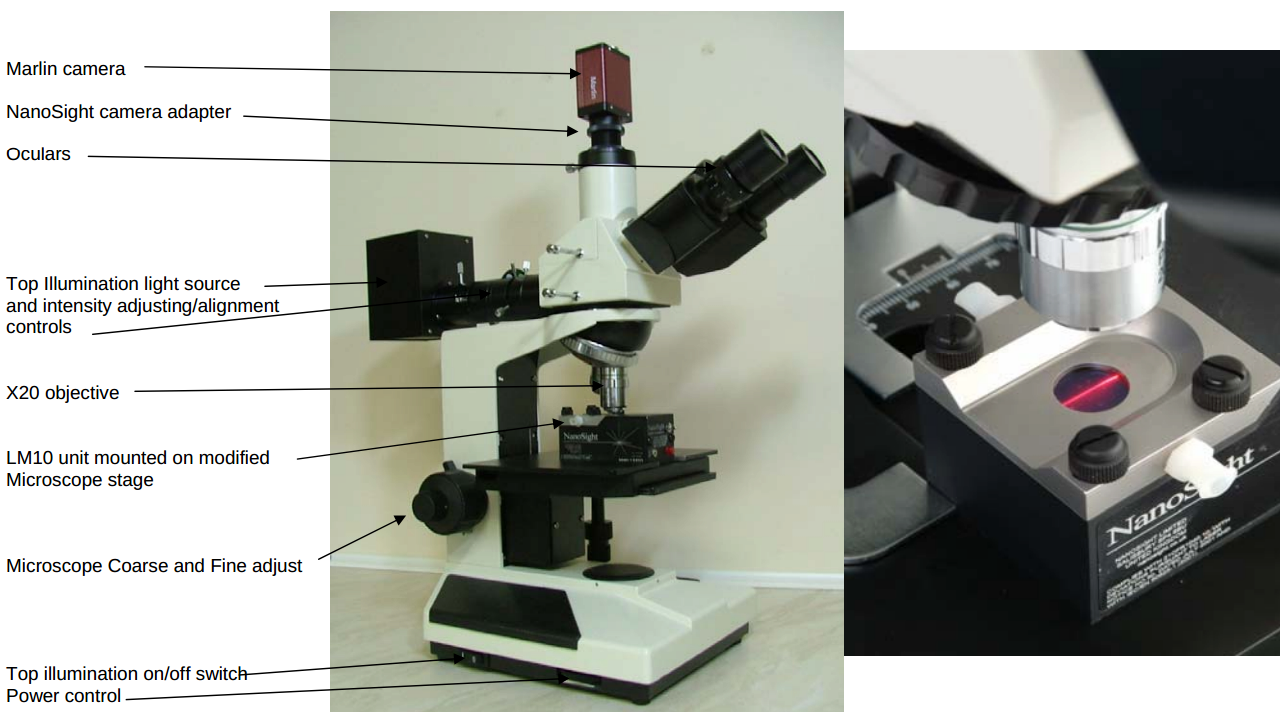
\includegraphics[width=\textwidth]{mikro2.png}
\caption{Mikroskop mit CCD-Kamera, Versuchszelle und LASER} \label{aufbau}
\end{figure}
Die Messzelle enthält die zu untersuchenden  $\unit[500]{\mu l}$ Suspension. Sie lässt sich mittels Spritze über Ein- und Auslaufstuzen reinigen, befüllen und entleeren. In ihr integriert ist bereits ein Einmoden-Diodenlaser der Klasse 1 ($P\unit[<20]{mW}$; $\lambda=\unit[655]{nm}$). Die aufgesetzte CCD-Kamera erfasst durch das Mikroskop die, vom LASER-Strahl getroffenen, propagierenden Partikel. Durch den Mikroskoptisch kann eine Scharfstellung des Bildes erfolgen, sowie ein geeigneter Bereich für die Aufnahme ausgewählt werden. Die Daten der Kamera werden von einer propiertären Software ausgewertet und grafisch bzw. in Echtzeit unverändert dargestellt.
\subsection{Versuchsablauf}
Mit dem Beschriebenen Aufbau werden 2 unterschiedliche Kaffeelösungen untersucht. Die betrachteten Partikel befinden sich im Nanometerbereich.\\
Für die Verifizierung der Zusammenhänge werden bei, einer möglichst konstanten Temperatur, sowohl Konzentrationen als auch Aufnahmedauern verändert. Beachtet werden muss jedoch, das polydisperse Lösungen vorliegen.\\
In der Software können Kontrast und weitere Kameraeinstellung bearbeitet werden, sodass ein möglichst gutes Bild mit wenigen '\tilt{toten}' Teilchen (Partikel, deren tracking nicht über die gesammte Aufnahme oder nur über ein paar \tilt{frames} betrieben werden kann) aufgenommen wird. Weiterhin ist es wichtig, eine nicht zu hohe Konzentration und zu kurze Aufnahmedauer auszuwählen, da die Leistung der Kamera und der Software begrenzt sind. Schließlich nimmt das Programm der \textbf{NANOSIGHT Ltd.} alle Berechnungen und Bestimmungen intern vor und liefert die gesuchten Daten.
\section{Auswertung}
\subsection{Diskussion}
\section{Anhang}
Die originalen Messwert-Aufzeichnungen liegen bei.
\end{document}